\documentclass{article}


% if you need to pass options to natbib, use, e.g.:
\PassOptionsToPackage{numbers, compress}{natbib}
% before loading neurips_2023


% ready for submission
% \usepackage{neurips_2023}


% to compile a preprint version, e.g., for submission to arXiv, add add the
% [preprint] option:
% \usepackage[preprint]{neurips_2023}


% to compile a camera-ready version, add the [final] option, e.g.:
\usepackage[final]{neurips_2023}


% to avoid loading the natbib package, add option nonatbib:
% \usepackage[nonatbib]{neurips_2023}


\usepackage[utf8]{inputenc} % allow utf-8 input
\usepackage[T1]{fontenc}    % use 8-bit T1 fonts
\usepackage{hyperref}       % hyperlinks
\usepackage{url}            % simple URL typesetting
\usepackage{booktabs}       % professional-quality tables
\usepackage{amsfonts}       % blackboard math symbols
\usepackage{nicefrac}       % compact symbols for 1/2, etc.
\usepackage{microtype}      % microtypography
\usepackage{xcolor}         % colors

\title{Surface Representation for Protein Binding Site Prediction}


% The \author macro works with any number of authors. There are two commands
% used to separate the names and addresses of multiple authors: \And and \AND.
%
% Using \And between authors leaves it to LaTeX to determine where to break the
% lines. Using \AND forces a line break at that point. So, if LaTeX puts 3 of 4
% authors names on the first line, and the last on the second line, try using
% \AND instead of \And before the third author name.


\author{%
  Shouchen Zhou\\
  ShanghaiTech University\\
  2021533042\\
  \texttt{zhoushch@shanghaitech.edu.cn} \\
  \And
  Mingzheng Wu \\
  ShanghaiTech University\\
  2021533066\\
  \texttt{wumzh@shanghaitech.edu.cn} \\
  \And
  Jiarui Xu \\
  ShanghaiTech University\\
  2021533092\\
  \texttt{xujr@shanghaitech.edu.cn} \\
}


\begin{document}


\maketitle

\begin{abstract}
Protein is the main carrier of life activities, and predicting protein binding sites can better help us predict protein function. In this project, we introduce the Laplace-Beltrami Surface Representation (LBSR) learning framework for protein binding site prediction. This pioneering approach leverages the Laplace-Beltrami eigenfunctions associated with a molecule's surface to formulate its representation, placing it within a 2D Riemannian manifold. LBSR furnishes a multi-resolution representation that adeptly captures both the geometric and chemical features of molecules. Furthermore, we introduce a harmonic message-passing mechanism, facilitating efficient spectral message propagation across the surface manifold. Our proposed method proves competitive with contemporary state-of-the-art deep learning models in ligand-binding protein pocket classification, underscoring its versatility and effectiveness in the domain of molecular representation learning.
  
\end{abstract}
\section{Introduction}
Understanding 3D environments is a fundamental objective shared by both the fields of Computer Vision (CV) and Computer Graphics (CG).
When presented with a point cloud, the primary aim is to discern its semantics, functionalities, and physical attributes.
An ideal molecular representation should well integrate both geometric (e.g., 3D conformation) and chemical information (e.g., electrostatic potential), contribute to its pocket type identification (semantics), dynamic features analysis (chem-physical properties), and docking (function).

Geometric deep learning (GDL) is now widely used in molecular representation learning, employing neural message passing on structures like 2D/3D molecular graphs, voxels, and point clouds to extract atomic-level features and elevate them to high-level features, similar to NeRF's\cite{nerfpytorch} input encoding. 

Nonetheless, we argue that such a design may not be the optimal representation for molecules. Current GDL methods often require equivariant networks to ensure proper transformation upon rotation and translation, potentially limiting the network's expressiveness. Secondly, current bottom-up learning approaches in GDL struggle to provide features at varying resolutions for different tasks. Thirdly, existing Graph Neural Networks (GNNs) mainly consider graph topology and overlook the incorporation of 3D spatial information into the encoding process.

Therefore, we introduce the Laplace-Beltrami Surface Representation (LBSR) learning framework which employs Laplace-Beltrami decomposition on the molecular surface \cite{shape-dna}.

The LBSR learning framework presents several benefits. First, it operates on a 2D Riemannian manifold rather than traditional 3D Euclidean space, inherently providing roto-translation invariance in molecular representation. Second, its top-down approach for representing molecules offers multi-resolution features, making it adaptable for a wide range of target molecules, from small compounds to large proteins. Lastly, LBSR effectively combines geometric and chemical features: the molecular shape forms the Riemannian manifold and atomic configurations dictate the functions on this manifold, ensuring a detailed and thorough representation of molecules.


To showcase the capability of our method, we applied the proposed techniques to address a problem related to drug discovery: ligand-binding protein pocket classification.
Our method exceeded the performance of current state-of-the-art deep learning models in classifying protein pockets.

\begin{figure*}[ht]
    \centering
    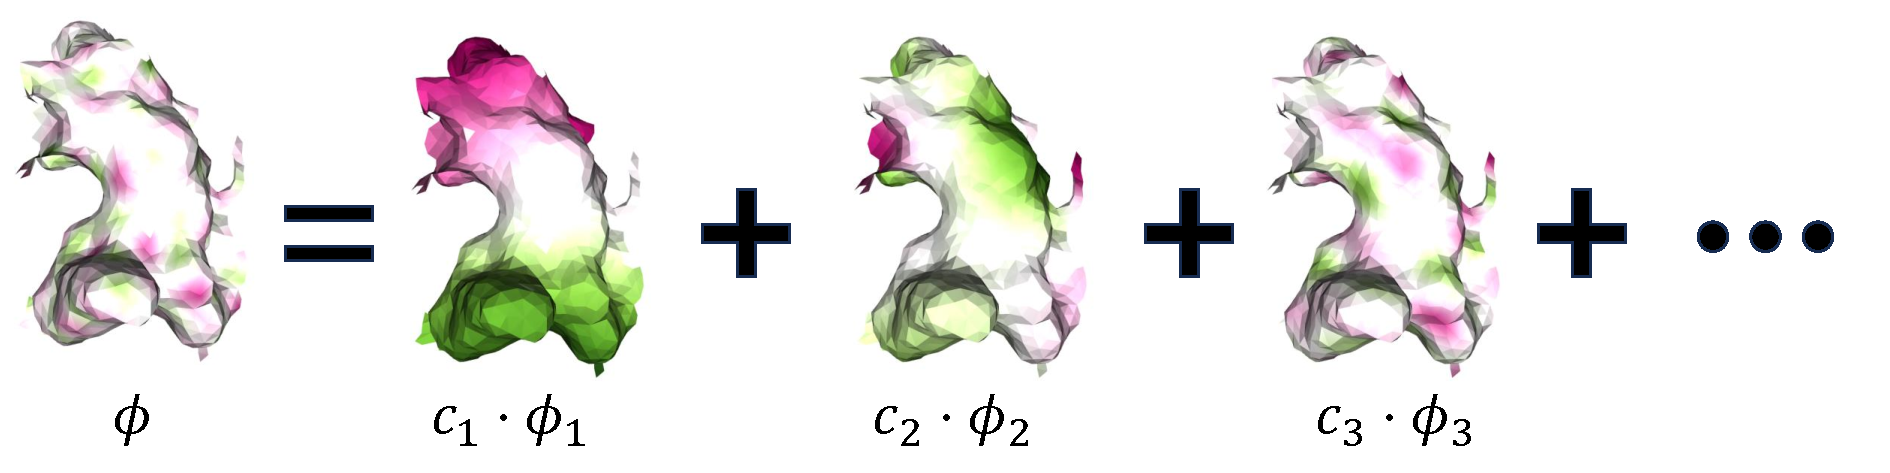
\includegraphics[width=0.7\linewidth]{figures/Laplace-Beltrami.pdf}
    \caption{
        The schematic diagram of the Laplace-Beltrami decomposition of the electrostatics field on a protein surface. It involves breaking down a continuous real-valued function $\phi$ into a linear combination of eigenfunctions $\phi_i$ with coefficients $c_i$. Eigenfunctions have varying spatial resolutions and are corresponding to distinctive details captured by them.
    }
    \label{fig:Laplace-Beltrami}
\end{figure*}

\section{Method}

\begin{figure}[htp]
    \centering
    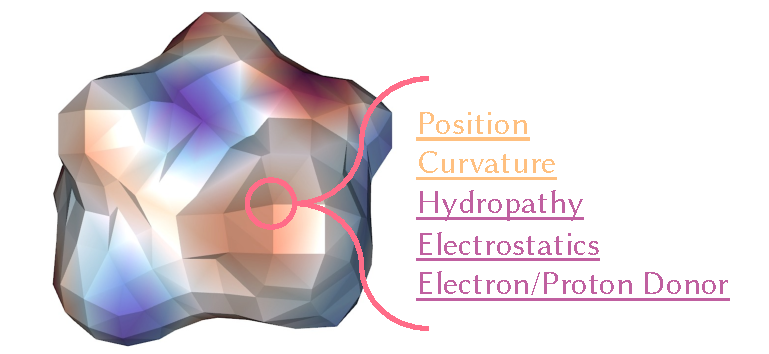
\includegraphics[width=0.5\linewidth]{figures/features.pdf}
    \caption{
        During the data pre-processing phase, we assign each vertex to the molecule's solvent-accessible surface area (SASA) with a total of five features: two geometrical (orange) and three chemical (purple) features.
        Some of these features are then decomposed by the Laplace-Beltrami operator to further exploit the intrinsic geometric and chemical properties of the molecular surface.
    }
    \label{fig:feature}
\end{figure}

Here we outline our data pre-processing approach, particularly emphasizing the computation of features on the molecule's solvent-accessible surface area.

\subsection{Data Pre-processing}

\paragraph{Solvent Accessible Surface}
The solvent-accessible surface area (SASA) describes the water-tight surface area of a biomolecule that is accessible to a solvent.
The solvent-accessible surface area (SASA) is depicted by the center of a solvent molecule, often modeled as a sphere (like a water molecule), as it traverses the surface of the biomolecule.
We use the \texttt{MSMS} \cite{MSMS} software that converts PDB in the point cloud format into the SAS in mesh format.

\paragraph{Features of Molecule}
The SASA of a molecule provides positional information, but this alone is insufficient for thorough network learning. To achieve a comprehensive understanding, it's essential to incorporate both geometric and chemical features in MaSIF\cite{MaSIF}.

For every vertex of the SASA, we attribute two geometric characteristics (position and curvature) and three chemical attributes (hydropathy index, continuum electrostatics, and the positions of free electrons and proton donors) to it, as depicted in Figure\ref{fig:feature}.

\paragraph{Geometric Features}
The position of each vertex has already been stored in the SASA.
Based on the mesh data, we use the libigl package to calculate the mean and Gaussian curvatures, which are then transformed to the principal curvatures, denoted as $\kappa_1$ and $\kappa_2$ with $\kappa_1>\kappa_2$.
Following MaSIF \cite{MaSIF}, these principal curvatures are then transformed to a range of $(-1, 1)$ with following formula
\begin{equation}
    \frac{2}{\pi}\arctan\frac{\kappa_1+\kappa_2}{\kappa_1-\kappa_2}
\end{equation}
where $-1$ denotes the most concave and $1$ the most convex.

\paragraph{Chemical Features}
We obtain each chemical feature from previous works and relevant software. For the hydropathy index, we consult Kyte and Doolittle's scale table for the 20 amino acid side chains \cite{hydropathy}.
For the continuum electrostatics, we use \texttt{PDB2PQR} \cite{PDB2PQR} to add hydrogen atoms to protein structures in PDB format.
Then, we use \texttt{APBS} \cite{APBS} to calculate the Poisson–Boltzmann electrostatics for each protein.

For the location of free electrons and proton donors, we follow the methodology derived from MaSIF\cite{MaSIF}, which assigns each vertex a value based on its proximity to the nearest heavy atom.

\begin{figure*}
    \centering
    % 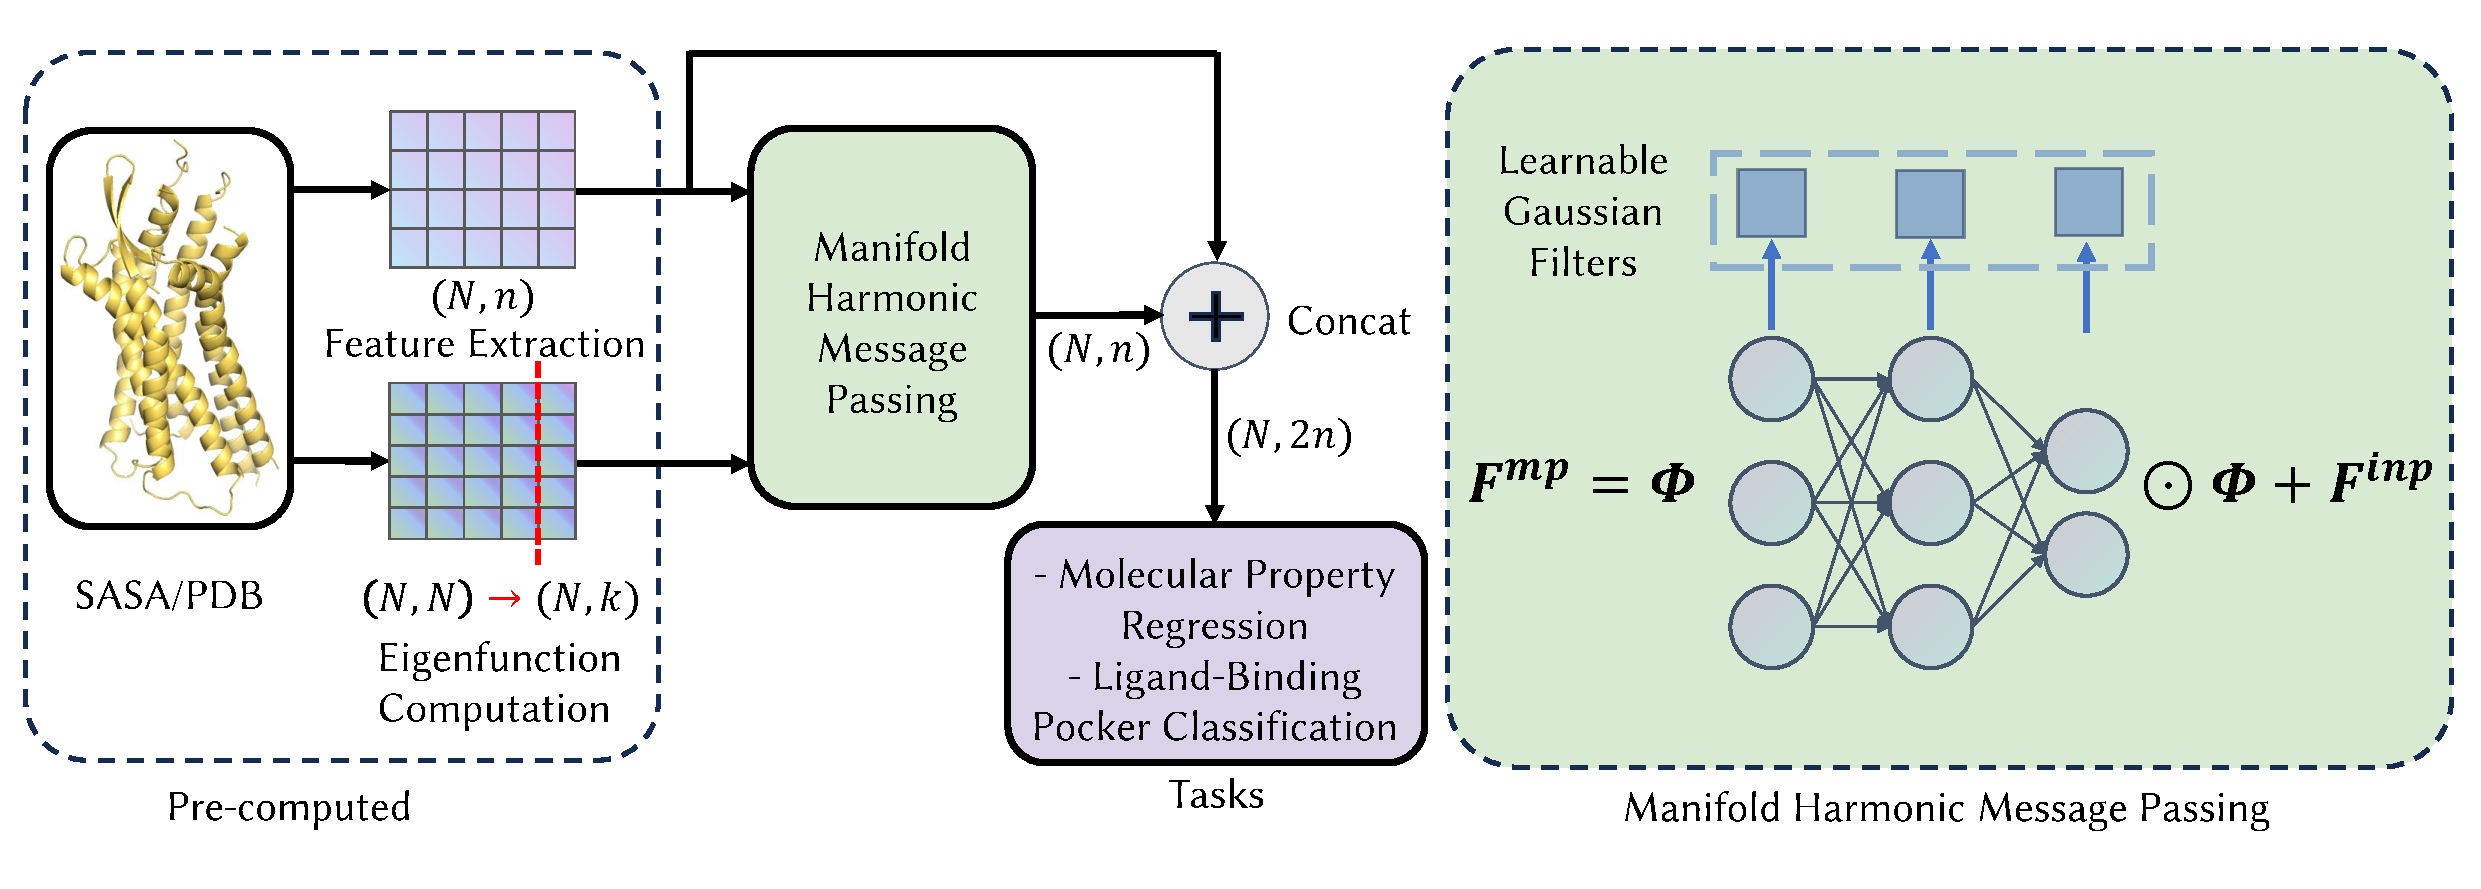
\includegraphics[width=\linewidth]{figures/pipeline.pdf}
    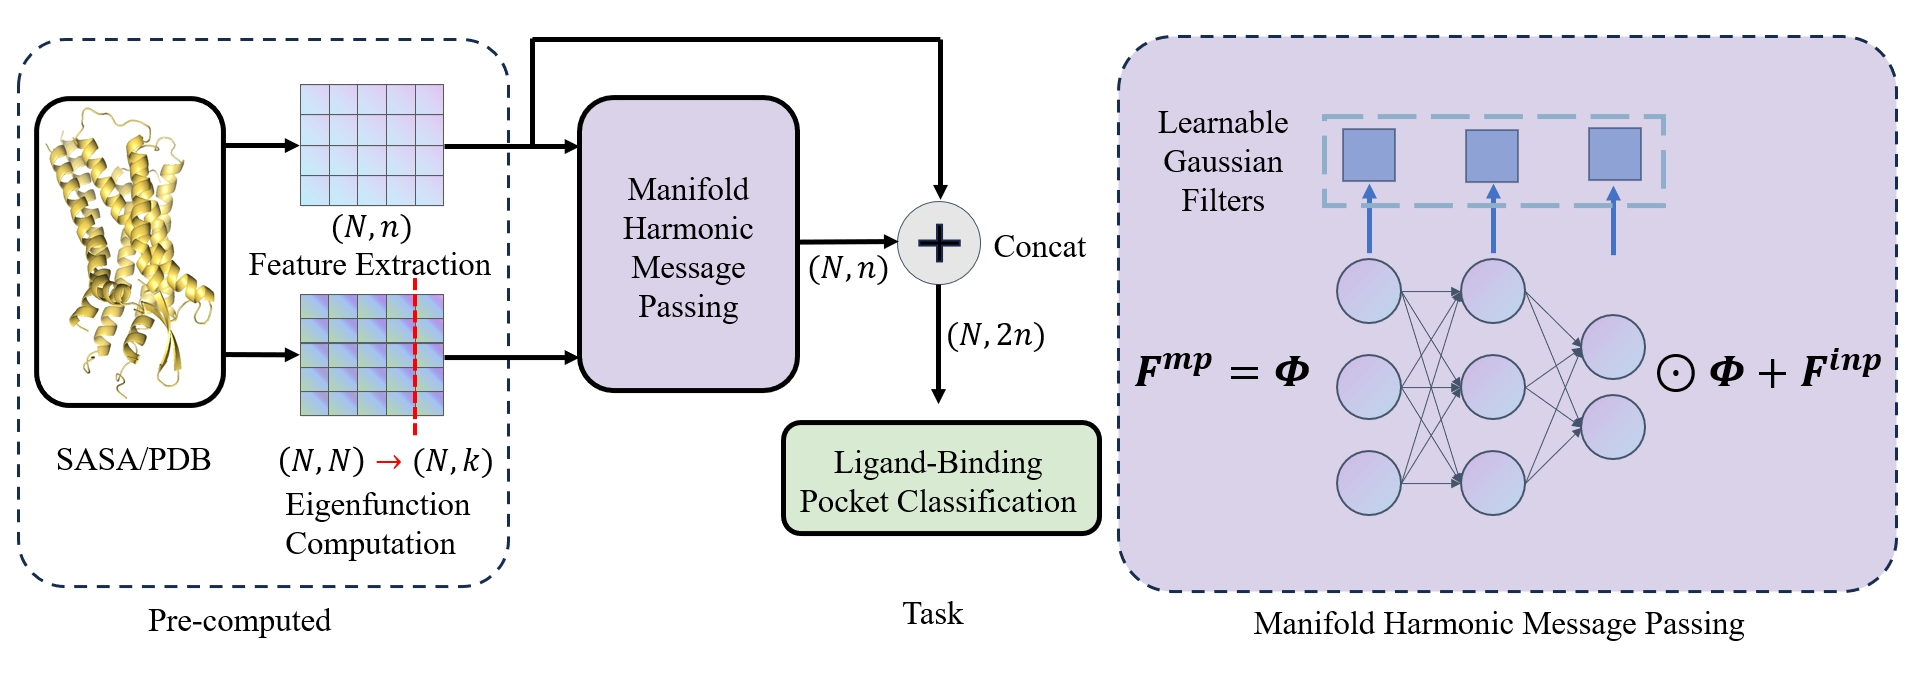
\includegraphics[width=\linewidth]{figures/pipeline.jpg}
    \caption{
        Pipeline.
        Given a protein surface SASA with $N$ vertices, we keep the first $k$ Laplace-Beltrami eigenfunctions with the truncated ascending eigenvalues.
        Then these eigenfunctions are sent into the Manifold Harmonic Message Passing module, which is primarily a fully connected network with the Heat Kernel Signatures.
        The output of the Manifold Harmonic Message Passing module is concatenated with features and sent to the downstream tasks, such as ligand-binding pocket classification.
    }
    \label{fig:pipeline}
\end{figure*}

\subsection{Laplace–Beltrami Decomposition}

To further exploit the features of the molecule's SASA, we apply the Laplace–Beltrami decomposition technique.
Intuitively, each feature is treated as a continuous real-valued function defined on the SASA, which is akin to a 2D manifold.
Similar to the Fourier transform, utilizing a series of orthonormal basis functions, denoted as $\{\phi_i\}$, to decompose the target function.
The basis functions are defined by the equation:
\begin{equation}
    \Delta\phi_i=\lambda_i\phi_i
\end{equation}
where $\Delta=-\nabla\cdot\nabla$ represents the Laplacian operator defined on the manifold.
$\lambda_i$ is the corresponding eigenvalue of $\phi_i$ arranged in ascending order, that is, $0\le\lambda_0\le\lambda_1\le\cdots$.
Figure \ref{fig:Laplace-Beltrami} shows the Laplace-Beltrami decomposition of the electrostatics field defined on a protein surface.

For a discrete surface mesh with $N$ vertices, the application of the Laplace-Beltrami decomposition results in the generation of $N$ eigenfunctions,
Each of these consists of $N$ values.
Therefore, this process yields a $N\times N$ eigenfunction matrix and $N\times 1$ eigenvalue matrix.
However, the complete utilization of this matrix significantly escalates computational costs.

To optimize this, a common strategy is to keep only the first $k$ eigenfunctions.
In our method, $k$ is selected differently for each downstream task.
The Laplace-Beltrami decomposition is done by \texttt{scipy}, following \texttt{HMR} \cite{HMR}.

We then transform the retained eigenfunctions and eigenvalues into the input for the downstream task, that is, ligand-binding pocket classification, using a fully connected network are concatenated with features extracted in the previous stage, as illustrated in figure \ref{fig:pipeline}.
\section{Experiments}

We subsequently apply our method to ligand-binding pocket classification, a $7$-classification task. The loss function was selected to be the cross-Entropy loss.

\begin{figure}[htp]
    \centering
    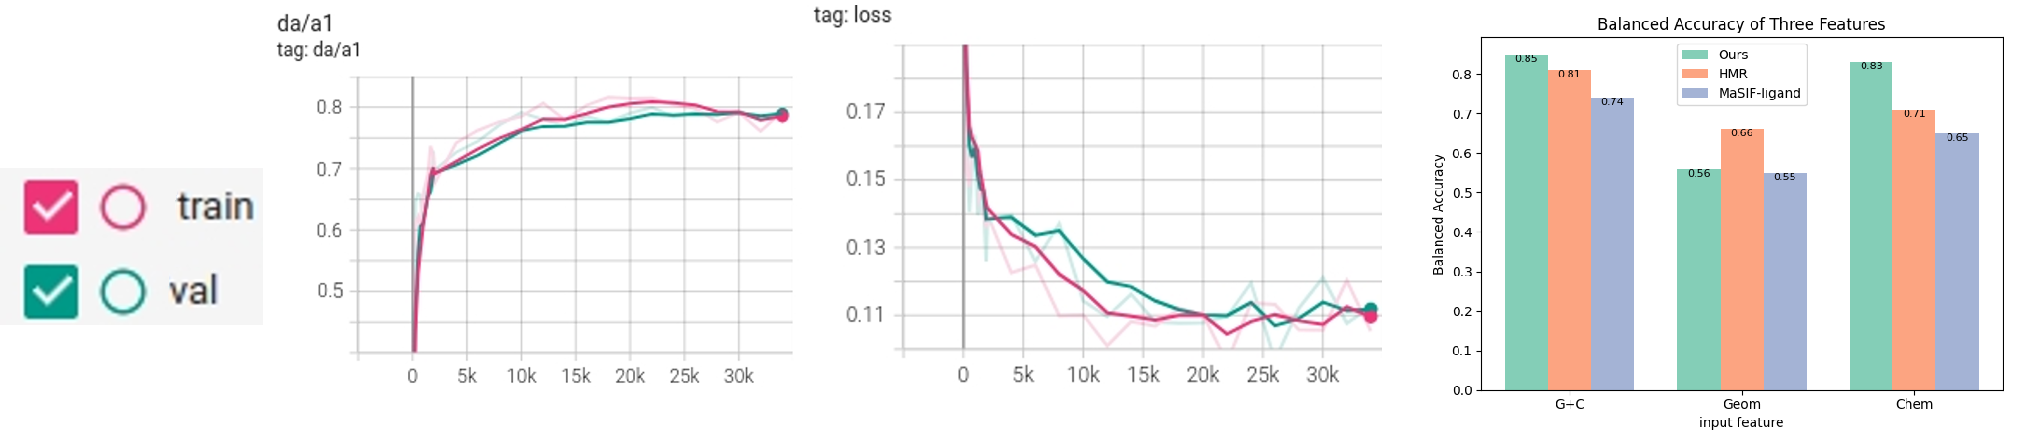
\includegraphics[width=\linewidth]{figures/result.png}
    \caption{
        Balanced accuracy of ligand-binding protein pocket classification.
        Models with different input features are compared: ``G+C'' indicates both geometric and chemical features.
    }
    \label{fig:ligand-binding-result}
\end{figure}

The dataset provided in MaSIF \cite{MaSIF} comprises computed properties of protein surfaces, crucial for understanding protein interactions with other molecules. These properties are utilized to discern patterns or "fingerprints" of interaction based on geometric and chemical features of the molecular surface. These fingerprints are then employed to predict how a given protein might interact with other proteins, ligands, or pharmaceuticals, enhancing insights into biological processes and assisting in drug design. Specifically, each protein in the dataset is associated with a preferred ligand-binding type among seven options (ADP, COA, FAD, HEM, NAD, NAP, and SAM). We consider the hydrophobicity score and partial charge as chemical features and mean/Gaussian curvature and Heat Kernel Signatures as geometric features. The dataset comprises 1634 training cases, 202 validation cases, and 418 testing cases.
\paragraph{Model Architecture}
Model Architecture and Performance 
The LBSR-based classification method contains 6 propagation layers followed by a global average pooling layer to aggregate information from all surface points of a ligand-binding pocket. A simple two-layer MLP is used to classify pockets into one of the seven ligand-binding pockets mentioned above.
LBSR has been trained to minimize the cross-entropy loss for 400 epochs and the one with the best balanced accuracy score on the validation set is selected.
\paragraph{Results}
Our result is shown in Figure \ref{fig:ligand-binding-result}. It suggests that our representation outperforms the 3D CNN-based methods used in MaSIF \cite{MaSIF}. It effectively encodes both the geometric and chemical features to predict protein binding type classification.
\section{Discussion}

We introduce an innovative framework, referred to as Laplace-Beltrami Surface Representation (LBSR), for generating molecular representations from surface manifolds. This novel approach combines geometric and chemical attributes represented as functions on the molecular surface manifold, utilizing harmonic message passing in the spectral domain. By integrating these attributes, we can capture molecular representations at different resolutions. Our LBSR method demonstrates promising results in protein pocket classification.

\paragraph{Limitation}

Our approach primarily emphasizes surfaces over volumes, assuming biomolecules possess rigid surfaces. However, achieving a more detailed modeling of biomolecules is possible. Adopting a quantum chemistry perspective could enhance system precision. Additionally, compared to graph neural networks based on atomic 3D coordinates, our surface-oriented approach lacks modeling of chemical bond information. Finally, extensive preprocessing significantly limits our method's speed. Consequently, we intend to advance our research in these directions.

\newpage
{
\small
\bibliography{ref}
\bibliographystyle{plainnat}
}

%%%%%%%%%%%%%%%%%%%%%%%%%%%%%%%%%%%%%%%%%%%%%%%%%%%%%%%%%%%%


\end{document}